\documentclass[]{article}
\usepackage{lmodern}
\usepackage{amssymb,amsmath}
\usepackage{ifxetex,ifluatex}
\usepackage{fixltx2e} % provides \textsubscript
\ifnum 0\ifxetex 1\fi\ifluatex 1\fi=0 % if pdftex
  \usepackage[T1]{fontenc}
  \usepackage[utf8]{inputenc}
\else % if luatex or xelatex
  \ifxetex
    \usepackage{mathspec}
    \usepackage{xltxtra,xunicode}
  \else
    \usepackage{fontspec}
  \fi
  \defaultfontfeatures{Mapping=tex-text,Scale=MatchLowercase}
  \newcommand{\euro}{€}
\fi
% use upquote if available, for straight quotes in verbatim environments
\IfFileExists{upquote.sty}{\usepackage{upquote}}{}
% use microtype if available
\IfFileExists{microtype.sty}{%
\usepackage{microtype}
\UseMicrotypeSet[protrusion]{basicmath} % disable protrusion for tt fonts
}{}
\usepackage[margin=1in]{geometry}
\usepackage{color}
\usepackage{fancyvrb}
\newcommand{\VerbBar}{|}
\newcommand{\VERB}{\Verb[commandchars=\\\{\}]}
\DefineVerbatimEnvironment{Highlighting}{Verbatim}{commandchars=\\\{\}}
% Add ',fontsize=\small' for more characters per line
\newenvironment{Shaded}{}{}
\newcommand{\KeywordTok}[1]{\textcolor[rgb]{0.00,0.44,0.13}{\textbf{{#1}}}}
\newcommand{\DataTypeTok}[1]{\textcolor[rgb]{0.56,0.13,0.00}{{#1}}}
\newcommand{\DecValTok}[1]{\textcolor[rgb]{0.25,0.63,0.44}{{#1}}}
\newcommand{\BaseNTok}[1]{\textcolor[rgb]{0.25,0.63,0.44}{{#1}}}
\newcommand{\FloatTok}[1]{\textcolor[rgb]{0.25,0.63,0.44}{{#1}}}
\newcommand{\CharTok}[1]{\textcolor[rgb]{0.25,0.44,0.63}{{#1}}}
\newcommand{\StringTok}[1]{\textcolor[rgb]{0.25,0.44,0.63}{{#1}}}
\newcommand{\CommentTok}[1]{\textcolor[rgb]{0.38,0.63,0.69}{\textit{{#1}}}}
\newcommand{\OtherTok}[1]{\textcolor[rgb]{0.00,0.44,0.13}{{#1}}}
\newcommand{\AlertTok}[1]{\textcolor[rgb]{1.00,0.00,0.00}{\textbf{{#1}}}}
\newcommand{\FunctionTok}[1]{\textcolor[rgb]{0.02,0.16,0.49}{{#1}}}
\newcommand{\RegionMarkerTok}[1]{{#1}}
\newcommand{\ErrorTok}[1]{\textcolor[rgb]{1.00,0.00,0.00}{\textbf{{#1}}}}
\newcommand{\NormalTok}[1]{{#1}}
\ifxetex
  \usepackage[setpagesize=false, % page size defined by xetex
              unicode=false, % unicode breaks when used with xetex
              xetex]{hyperref}
\else
  \usepackage[unicode=true]{hyperref}
\fi
\hypersetup{breaklinks=true,
            bookmarks=true,
            pdfauthor={},
            pdftitle={Parametryczna postać czasu do nawrotu choroby w leczeniu raka piersi},
            colorlinks=true,
            citecolor=blue,
            urlcolor=blue,
            linkcolor=magenta,
            pdfborder={0 0 0}}
\urlstyle{same}  % don't use monospace font for urls
\setlength{\parindent}{0pt}
\setlength{\parskip}{6pt plus 2pt minus 1pt}
\setlength{\emergencystretch}{3em}  % prevent overfull lines
\setcounter{secnumdepth}{0}

%%% Use protect on footnotes to avoid problems with footnotes in titles
\let\rmarkdownfootnote\footnote%
\def\footnote{\protect\rmarkdownfootnote}

%%% Change title format to be more compact
\usepackage{titling}
\setlength{\droptitle}{-2em}
  \title{Parametryczna postać czasu do nawrotu choroby w leczeniu raka piersi}
  \pretitle{\vspace{\droptitle}\centering\huge}
  \posttitle{\par}
  \author{}
  \preauthor{}\postauthor{}
  \date{}
  \predate{}\postdate{}


\usepackage{polski}
\usepackage[T1]{fontenc}
\usepackage[utf8]{inputenc} 
%\usepackage[top=1.5cm, bottom=1.5cm, left=0.85cm, right=0.85cm]{geometry}
\usepackage{fancyhdr}
\pagestyle{fancy}
\fancyhead[RO,LE]{\bfseries \small{P. Auguścik, M. Kosiński, B. Sozańska, A. Szewczyk}}
\fancyhead[RE,LO]{\bfseries \small{Biostatystyka, Projekt nr 2}}
\AtBeginDocument{\thispagestyle{fancy}}
\usepackage{rotating}
\usepackage{subfigure}
\usepackage{pdflscape}

\usepackage{amsfonts}
\usepackage{amsmath}
\usepackage{amssymb}
\usepackage{color}
\usepackage{amsthm}
\usepackage{longtable}
\usepackage{wrapfig,booktabs}
\usepackage{tikz}
\usepackage{float}
\usepackage{hyperref} %pakiet do dodawania hiperłącz
\hypersetup{colorlinks=true,
            linkcolor=black,
            citecolor=black,
            urlcolor=black}
%\title{\textbf{\LARGE{Biostatystyka - Projekt zaliczeniowy bardzo fajny} }}


\begin{document}

\maketitle


\thispagestyle{fancy}

Chcąc sprawdzić, jakie czynniki mają istotnie statystyczny wpływ na czas
do zdarzenia jakim jest zgon przy analizie danych dotyczących raka
piersi, zaproponowano sprawdzenie czy modele parametryczne zakładające
postać rozkładu czasu do zdarzenia są adekwatne w danym problemie
medycznym.

\textbf{Wybór parametrycznej formy modelu.}

Sprawdzając postać parametryczną dla modelu AFT postanowiono wybrać
rozkład z bogatej rodziny uogólnionych rozkładów F. Korzystając z
pakietu \texttt{flexsurv} dopasowano modele Weibulla, Log-logistyczny,
\text{Log-normalny}, Uogólniony Gamma oraz Uogólniony F.

\begin{Shaded}
\begin{Highlighting}[]
\NormalTok{AFT.GG <-}\StringTok{ }\KeywordTok{flexsurvreg}\NormalTok{(}\KeywordTok{Surv}\NormalTok{(rectime,censrec)~horm+prog+estr+}\KeywordTok{as.factor}\NormalTok{(grade)+meno+size+nodes, }
                             \DataTypeTok{data =} \NormalTok{dane, }\DataTypeTok{dist=}\StringTok{"gengamma"}\NormalTok{)}
\NormalTok{AFT.GF <-}\StringTok{ }\KeywordTok{flexsurvreg}\NormalTok{(}\KeywordTok{Surv}\NormalTok{(rectime,censrec)~horm+prog+estr+}\KeywordTok{as.factor}\NormalTok{(grade)+meno+size+nodes, }
                             \DataTypeTok{data =} \NormalTok{dane, }\DataTypeTok{dist=}\StringTok{"genf"}\NormalTok{)}
\NormalTok{AFT.LL <-}\StringTok{ }\KeywordTok{flexsurvreg}\NormalTok{(}\KeywordTok{Surv}\NormalTok{(rectime,censrec)~horm+prog+estr+}\KeywordTok{as.factor}\NormalTok{(grade)+meno+size+nodes, }
                             \DataTypeTok{data =} \NormalTok{dane, }\DataTypeTok{dist=}\StringTok{"genf"}\NormalTok{, }\DataTypeTok{inits=}\KeywordTok{c}\NormalTok{(}\DecValTok{3}\NormalTok{,}\FloatTok{0.2}\NormalTok{,}\DecValTok{0}\NormalTok{,}\DecValTok{1}\NormalTok{,}\DecValTok{0}\NormalTok{,}\DecValTok{0}\NormalTok{,}\DecValTok{0}\NormalTok{,}\DecValTok{0}\NormalTok{,}\DecValTok{0}\NormalTok{,}\DecValTok{0}\NormalTok{,}\DecValTok{0}\NormalTok{,}\DecValTok{0}\NormalTok{), }
                             \DataTypeTok{fixedpars =} \KeywordTok{c}\NormalTok{(}\DecValTok{3}\NormalTok{,}\DecValTok{4}\NormalTok{))}
\NormalTok{AFT.Weibull <-}\StringTok{ }\KeywordTok{flexsurvreg}\NormalTok{(}\KeywordTok{Surv}\NormalTok{(rectime,censrec)~horm+prog+estr+}\KeywordTok{as.factor}\NormalTok{(grade)+meno+}
\StringTok{                             }\NormalTok{size+nodes,}
                             \DataTypeTok{data =} \NormalTok{dane, }\DataTypeTok{dist=}\StringTok{"weibull"}\NormalTok{)}
\NormalTok{AFT.LN <-}\StringTok{ }\KeywordTok{flexsurvreg}\NormalTok{(}\KeywordTok{Surv}\NormalTok{(rectime,censrec)~horm+prog+estr+}\KeywordTok{as.factor}\NormalTok{(grade)+meno+size+nodes, }
                             \DataTypeTok{data =} \NormalTok{dane, }\DataTypeTok{dist=}\StringTok{"lnorm"}\NormalTok{)}
\end{Highlighting}
\end{Shaded}

W celu oceny, który model jest adekwatny i wystarczający, przeprowdzono
testy ilorazu wiarogodności, jak poniżej.

Wartości logarytmów funkcji wiarogodności analizowanych modeli:

\begin{table}[hbt!]
\centering
\begin{tabular}{lr}
\toprule%
  & loglik\\ \toprule%

Gen Gamma & -2553.051\\

Gen F & -2553.067\\

Log-logistic & -2563.449\\

Weibull & -2575.998\\

Log-normal & -2555.798\\
\bottomrule
\end{tabular}
\caption{Wartości logarytmów funkcji wiarogodności dla modeli parametrycznych.}
\end{table}

P-wartości testów:

\begin{table}[hbt!]
\centering
\begin{tabular}{lr}
\toprule%
  & p-wartość\\
\toprule%
GF vs GG & 1.0000\\

GG vs LL & 0.0000\\

GG vs Wei & 0.0000\\

GG vs LN & 0.0641\\
\bottomrule
\end{tabular}
\caption{Wartości krytycze testów.}
\end{table}

Testując możliowść użycia danego rozkładu, najpierw przeprowadzono test
dla uogólnionego rozładu gamma \text{i uogólnionego} F. Stwierdzono, na
poziomie istotności \(\alpha=0.05\), po poprawce Bonferroniego
uwzględniającej 4 testy, czyli na poziomie istotności dla pojedycznego
testu równym \(\alpha_i = 0.0125, i =1,2,3,4\), że nie ma podstaw do
odrzucenia hipotezy zerowej w teście sprawdzającym czy model
\text{z mniejszej} rodziny uogólnionych rozkładów gamma jest właściwy w
porównaniu do modelu z większej rodziny uogólnionych rozkładów F.
Następnie dla rozkładu z uogólnionej rodziny rozkładów gamma
przeprowadzono 3 testy sprawdzające, czy modele z mniejszej rodziny
(log-normalny, log-logistyczny, Weibulla) są właściwe
\text{w porównaniu} do rozkładu z uogólnionej rodziny rozkładów gamma.
Tylko w przypadku rozkładu log-normalnego nie ma podstaw
\text{do odrzucenia} hipotezy, że ten rozkład jest właściwy w porównaniu
\text{do rozkładu} z szerszej rodziny rozkładów uogólnionych gamma. Dla
rozkładu log-logistycznego i Weibulla odrzucono hipotezę zerową o tym,
że te rozkłady są właściwe w stosunku do rozkładu z szerszej rodziny
rozkładów uogólnionych gamma.

Zatem w dalszej części raportu sprawdzamy dopasowanie modelu
log-normalnego.

\textbf{Sprawdzenie dopasowania modelu log-normalnego.}

\begin{figure}[hbt!]
  \vspace{-20pt}
  \begin{center}
     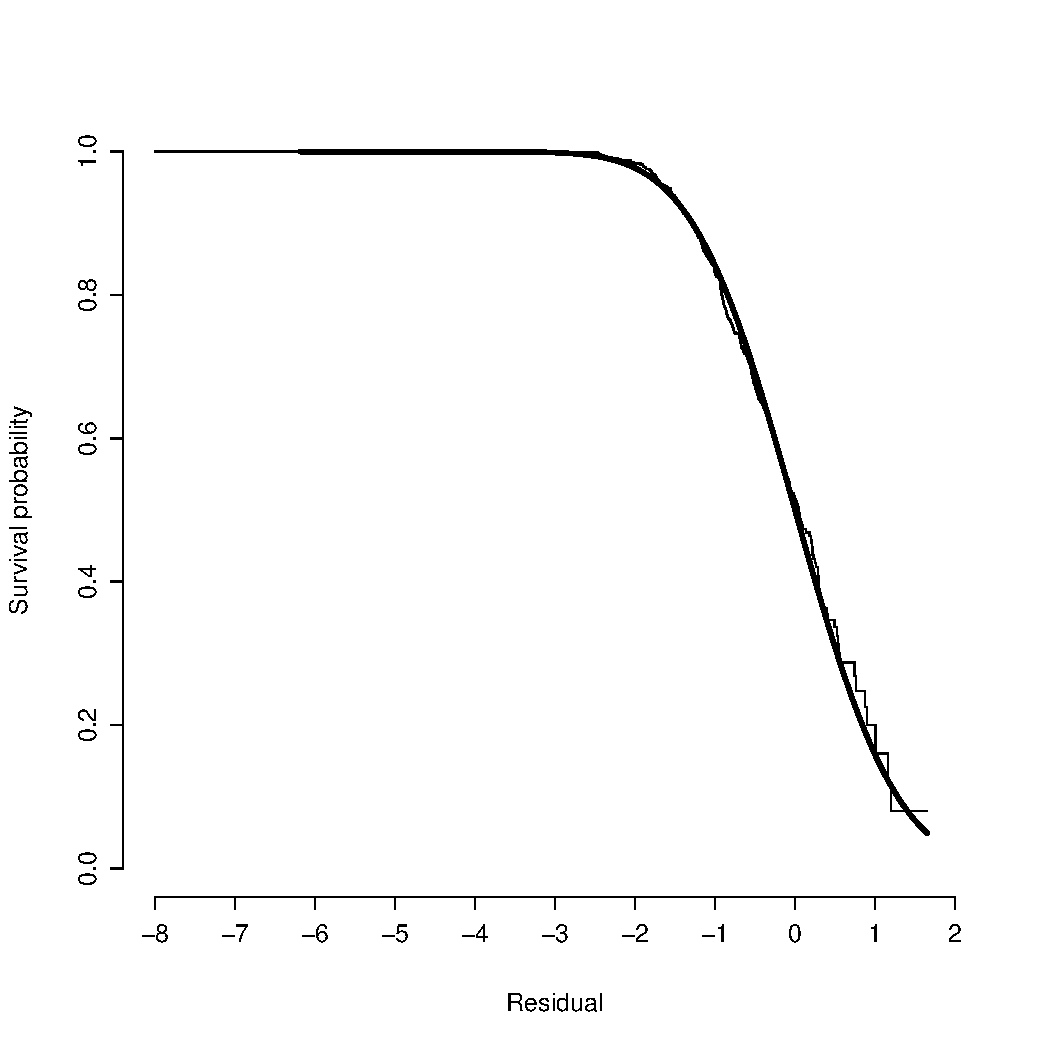
\includegraphics[width=0.7\textwidth, height=3in]{lognormal.pdf}
  \end{center}
  \vspace{-20pt}
  \label{fig:sc}
  \caption{Reszty modelu a cenzurowana próbka z rozkładu log-normalnego.}

\end{figure}

W następnym kroku zweryfikowano, czy reszty modelu zachowują się jak
cenzurowana próbka z rozkładu log-normalnego, co zostało pokazane na
Rysunku 1. Na podstawie wykresu widać, że nie ma widocznych odstępstw
między krzywymi, co może świadczyć o dobrym dopasowaniu modelu.
Parametryczne założenie, że reszty pochodzą z rozkładu log-normalnego
wydaje się być spełnione na podstawie \text{Rysunku 1.}

\textbf{ Podsumownie modelu log-normalnego.}

Podsumowanie modelu można uzyskać poleceniem jak poniżej:

\begin{Shaded}
\begin{Highlighting}[]
\KeywordTok{psm}\NormalTok{(}\KeywordTok{Surv}\NormalTok{(rectime,censrec)~horm+prog+estr+}\KeywordTok{as.factor}\NormalTok{(grade)+meno+size+nodes, }
        \DataTypeTok{data =} \NormalTok{dane, }\DataTypeTok{dist =} \StringTok{"lognormal"}\NormalTok{)}
\end{Highlighting}
\end{Shaded}

\begin{verbatim}

Parametric Survival Model: Log Normal Distribution

psm(formula = Surv(rectime, censrec) ~ horm + prog + estr + as.factor(grade) + 
    meno + size + nodes, data = dane, dist = "lognormal")

                    Model Likelihood     Discrimination    
                       Ratio Test           Indexes        
Obs         686    LR chi2     126.17    R2       0.168    
Events      299    d.f.             8    Dxy      0.382    
sigma 0.9690015    Pr(> chi2) <0.0001    g        0.036    
                                         gr       0.564    

            Coef    S.E.   Wald Z Pr(>|Z|)
(Intercept)  7.4967 0.2670 28.08  <0.0001 
horm         0.3339 0.0958  3.49  0.0005  
prog         0.4995 0.1097  4.55  <0.0001 
estr         0.0418 0.1083  0.39  0.6992  
grade=2     -0.4396 0.1643 -2.68  0.0075  
grade=3     -0.4780 0.1880 -2.54  0.0110  
meno        -0.0427 0.0932 -0.46  0.6469  
size        -0.0056 0.0031 -1.82  0.0685  
nodes       -0.0483 0.0080 -6.08  <0.0001 
Log(scale)  -0.0315 0.0443 -0.71  0.4773  
\end{verbatim}

Zmiennymi istotnymi w modelu są \texttt{horm}, \texttt{prog}, oba
poziomy zmiennej \texttt{grade} względem poziomu referencyjnego oraz
\texttt{nodes}. Współczynniki modelu dla tych zmiennych wynoszą
odpowiednio 0.3339, 0.4995, -0.4396, -0.4780, -0.0483. Oznacza to, że
czas do nawrotu choroby przy użyciu terapii hormonalnej jest dłuższy
\(e^{0.3339} = 1.4\) raza w porównaniu do sytuacji gdy nie jest
stosowana terapia hormonalna, przy założeniu stałości pozostałych
zmiennych. Czas do nawrotu choroby przy dodatnim wskaźniku progesteronu
jest dłuższy \(e^{0.4995} = 1.6\) raza w porównaniu do sytuacji, gdy
pacjentka posiada ujemny wskaźnik poziomu progesteronu, przy założeniu
stałości pozostałych zmiennych. Czas do nawrotu choroby przy średnim
stopniu zróżnicowania komórek nowotworu jest krótszy
\(e^{-0.4396} = 0.64\) raza w porównaniu do sytuacji, gdy pacjentka
posiada wysoki stopień zróżnicowania komórek nowotworu, przy założeniu
stałości pozostałych zmiennych. Natomiast, gdy pacjentka posiada niski
stopień zróżnicowania nowotworu, to czas do nawrotu choroby jest krótszy
\(e^{-0.4780} = 0.62\) raza w porównaniu do sytuacji gdy pacjentka
posiada wysoki stopień zróżnicowania komórek nowotworu, przy założeniu
stałości pozostałych zmiennych. Czas do nawrotu choroby przy wzroście
liczby węzłów chłonnych \text{z przerzutami} nowotworu o jeden jest
krótszy \(e^{-0.0483} = 0.95\) raza, przy założeniu stałości pozostałych
zmiennych.

\newpage
\textbf{Kody:}

\begin{Shaded}
\begin{Highlighting}[]
\KeywordTok{library}\NormalTok{(foreign)}
\NormalTok{dane <-}\StringTok{ }\KeywordTok{read.dta}\NormalTok{(}\StringTok{"gbcs_short.dta"}\NormalTok{)}
\KeywordTok{library}\NormalTok{(survival)}
\KeywordTok{library}\NormalTok{(flexsurv)}
\KeywordTok{library}\NormalTok{(rms)}

\CommentTok{#modele:}
\NormalTok{AFT.GG <-}\StringTok{ }\KeywordTok{flexsurvreg}\NormalTok{(}\KeywordTok{Surv}\NormalTok{(rectime,censrec)~horm+prog+estr+}\KeywordTok{as.factor}\NormalTok{(grade)+meno+size+nodes, }
                             \DataTypeTok{data =} \NormalTok{dane, }\DataTypeTok{dist=}\StringTok{"gengamma"}\NormalTok{)}
\NormalTok{AFT.GF <-}\StringTok{ }\KeywordTok{flexsurvreg}\NormalTok{(}\KeywordTok{Surv}\NormalTok{(rectime,censrec)~horm+prog+estr+}\KeywordTok{as.factor}\NormalTok{(grade)+meno+size+nodes, }
                             \DataTypeTok{data =} \NormalTok{dane, }\DataTypeTok{dist=}\StringTok{"genf"}\NormalTok{)}
\NormalTok{AFT.LL <-}\StringTok{ }\KeywordTok{flexsurvreg}\NormalTok{(}\KeywordTok{Surv}\NormalTok{(rectime,censrec)~horm+prog+estr+}\KeywordTok{as.factor}\NormalTok{(grade)+meno+size+nodes, }
                             \DataTypeTok{data =} \NormalTok{dane, }\DataTypeTok{dist=}\StringTok{"genf"}\NormalTok{, }\DataTypeTok{inits=}\KeywordTok{c}\NormalTok{(}\DecValTok{3}\NormalTok{,}\FloatTok{0.2}\NormalTok{,}\DecValTok{0}\NormalTok{,}\DecValTok{1}\NormalTok{,}\DecValTok{0}\NormalTok{,}\DecValTok{0}\NormalTok{,}\DecValTok{0}\NormalTok{,}\DecValTok{0}\NormalTok{,}\DecValTok{0}\NormalTok{,}\DecValTok{0}\NormalTok{,}\DecValTok{0}\NormalTok{,}\DecValTok{0}\NormalTok{), }
                      \DataTypeTok{fixedpars =} \KeywordTok{c}\NormalTok{(}\DecValTok{3}\NormalTok{,}\DecValTok{4}\NormalTok{))}
\NormalTok{AFT.Weibull <-}\StringTok{ }\KeywordTok{flexsurvreg}\NormalTok{(}\KeywordTok{Surv}\NormalTok{(rectime,censrec)~horm+prog+estr+}\KeywordTok{as.factor}\NormalTok{(grade)+meno+size+nodes, }
                              \DataTypeTok{data =} \NormalTok{dane, }\DataTypeTok{dist=}\StringTok{"weibull"}\NormalTok{)}
\NormalTok{AFT.LN <-}\StringTok{ }\KeywordTok{flexsurvreg}\NormalTok{(}\KeywordTok{Surv}\NormalTok{(rectime,censrec)~horm+prog+estr+}\KeywordTok{as.factor}\NormalTok{(grade)+meno+size+nodes, }
                              \DataTypeTok{data =} \NormalTok{dane, }\DataTypeTok{dist=}\StringTok{"lnorm"}\NormalTok{)}

\CommentTok{#Wartości logarytmów funkcji wiarogodności dla modeli:}
\KeywordTok{matrix}\NormalTok{( }\KeywordTok{c}\NormalTok{(AFT.GG$loglik, }\CommentTok{# loglik generalized G }
\NormalTok{AFT.GF$loglik, }\CommentTok{# loglik generalized F}
\NormalTok{AFT.LL$loglik, }\CommentTok{# logik log-logistic}
\NormalTok{AFT.Weibull$loglik, }\CommentTok{# logik Weibull}
\NormalTok{AFT.LN$loglik), }\DataTypeTok{ncol=}\DecValTok{1}\NormalTok{) ->x50 }\CommentTok{# logik log-normalny}
\KeywordTok{rownames}\NormalTok{(x50) <-}\StringTok{ }\KeywordTok{c}\NormalTok{(}\StringTok{"Gen Gamma"}\NormalTok{, }\StringTok{"Gen F"}\NormalTok{, }\StringTok{"Log-logistic"}\NormalTok{, }\StringTok{"Weibull"}\NormalTok{, }\StringTok{"Log-normal"}\NormalTok{)}
\KeywordTok{colnames}\NormalTok{(x50) <-}\StringTok{ "loglik"}

\CommentTok{#p-wartości testóW:}
\KeywordTok{matrix}\NormalTok{(}\KeywordTok{round}\NormalTok{(}\KeywordTok{c}\NormalTok{(}\DecValTok{1}\NormalTok{-}\KeywordTok{pchisq}\NormalTok{(}\DecValTok{2}\NormalTok{*(AFT.GF$loglik-AFT.GG$loglik),}\DecValTok{2}\NormalTok{),}
\DecValTok{1}\NormalTok{-}\KeywordTok{pchisq}\NormalTok{(}\DecValTok{2}\NormalTok{*(AFT.GG$loglik-AFT.LL$loglik),}\DecValTok{2}\NormalTok{),}
\DecValTok{1}\NormalTok{-}\KeywordTok{pchisq}\NormalTok{(}\DecValTok{2}\NormalTok{*(AFT.GG$loglik-AFT.Weibull$loglik),}\DecValTok{2}\NormalTok{), }
\DecValTok{1}\NormalTok{-}\KeywordTok{pchisq}\NormalTok{(}\DecValTok{2}\NormalTok{*(AFT.GG$loglik-AFT.LN$loglik),}\DecValTok{2}\NormalTok{)), }\DataTypeTok{digits=}\DecValTok{4}\NormalTok{), }\DataTypeTok{ncol=}\DecValTok{1}\NormalTok{) ->}\StringTok{ }\NormalTok{x65}
\KeywordTok{rownames}\NormalTok{(x65) <-}\StringTok{ }\KeywordTok{c}\NormalTok{(}\StringTok{"GF vs GG"}\NormalTok{, }\StringTok{"GG vs LL"}\NormalTok{, }\StringTok{"GG vs Wei"}\NormalTok{, }\StringTok{"GG vs LN"}\NormalTok{)}
\KeywordTok{colnames}\NormalTok{(x65) <-}\StringTok{ "p-wartość"}

\CommentTok{#Sprawdzenie dopasowania modelu log-normalnego}
\NormalTok{logNorx1 <-}\StringTok{ }\KeywordTok{psm}\NormalTok{(}\KeywordTok{Surv}\NormalTok{(rectime,censrec)~horm+prog+estr+}\KeywordTok{as.factor}\NormalTok{(grade)+meno+size+nodes, }
        \DataTypeTok{data =} \NormalTok{dane, }\DataTypeTok{dist =} \StringTok{"lognormal"}\NormalTok{) }
\NormalTok{res.LogN1 <-}\StringTok{ }\KeywordTok{resid}\NormalTok{(logNorx1,}\DataTypeTok{type=}\StringTok{"cens"}\NormalTok{)}

\KeywordTok{survplot}\NormalTok{(}\KeywordTok{npsurv}\NormalTok{(res.LogN1 ~}\DecValTok{1}\NormalTok{),}\DataTypeTok{conf=}\StringTok{"none"}\NormalTok{,}\DataTypeTok{ylab=}\StringTok{"Survival probability"}\NormalTok{, }\DataTypeTok{xlab=}\StringTok{"Residual"}\NormalTok{)}
\KeywordTok{lines}\NormalTok{(res.LogN1)}
\KeywordTok{dev.off}\NormalTok{()}
\end{Highlighting}
\end{Shaded}

\end{document}
